\chapter*{Ejercicio 56 Cápitulo 5 ABD}
\textbf{Sea $F(x)=\displaystyle \int_{0}^{x} \frac{t^2 - 3}{t^4 + 7} \, dt$}
\begin{enumerate}[label=\alph*)]
	\item[(a)] \textbf{Encuentra los intervalos en los cuales \( F \) está aumentando y aquellos en los cuales \( F \) está disminuyendo. }
	\item[(b)] \textbf{Encuentra los intervalos abiertos en los cuales \( F \) es cóncava hacia arriba y aquellos en los cuales \( F \) es cóncava hacia abajo. }
	\item[(c)] \textbf{Encuentra los valores de \( x \), si los hay, en los cuales la función \( F \) tiene extremos absolutos. }
	\item[(d)] \textbf{Usa un CAS para graficar \( F \), y confirma que los resultados en las partes (a), (b) y (c) son consistentes con la gráfica.}
\end{enumerate}
a) Regiones de crecimiento y decrecimiento
Encontremos los puntos críticos por la prueba de la primer derivada
Sabemos que, Por el teorema fundamental del cálculo
\begin{align*}
	\frac{dF}{dx}=\frac{x^2-3}{x^4+7}=0\iff & x^2-3=0        \\
	                                        & x^2=3          \\
	                                        & x=\pm \sqrt{3} \\
\end{align*}
El análisis de signos de los intervalos
\begin{table}[!hbt]
	\begin{center}
		\begin{tabular}{| c | c | c | c | c |}
			\hline
			\multicolumn{5}{ |c| }{Análisis de los intervalos}                                           \\ \hline
			intervalo                  & Punto de prueba & $f'(x)$            & signo & conclución       \\ \hline
			($-\infty,-\sqrt{3}\big]$  & -2              & $\frac{+}{+}     $ & +     & f es creciente   \\
			$[-\sqrt{3},\sqrt{3}\big]$ & 0               & $\frac{-}{+}     $ & -     & f es decreciente \\
			$[\sqrt{3},\infty$\big)    & 2               & $\frac{+}{+}     $ & +     & f es creciente   \\\hline
		\end{tabular}
		\caption{tabla de análsis de signos de las regiones de crecimiento y decrecimiento.}
		\label{tab: tabla de análsis de signos de las regiones de crecimiento y decrecimiento}
	\end{center}
\end{table}

$\implies$ El análisis nos dice que f es creciente en el intervalo ($-\infty,-\sqrt{3}\big]$, decreciente en el intervalo $[-\sqrt{3},\sqrt{3}\big]$ y creciente nuevamente en el intervalo $[\sqrt{3},\infty$).

				b) Análisis de concavidad.

				Por la prueba de la segunda derivada podemos hacer el análisis.
				\begin{align*}
					\frac{d^2F}{dt^2} & =\frac{(t^4+7)(2t)-(t^2-3)(4t^3)}{(t^4+7)^2}                                   \\
					                  & =\frac{2t((t^4+7)-2t^2(t^2-3))}{(t^4+7)^2}                                     \\
					                  & =\frac{-2t(-(t^4+7)+2t^2(t^2-3))}{(t^4+7)^2}                                   \\
					                  & =\frac{-2t(2t^2(t^2-3)-(t^4+7))}{(t^4+7)^2}                                    \\
					                  & =\frac{-2t(2t^4-6t^2-t^4-7)}{(t^4+7)^2}=0                                      \\
					                  & =\frac{-2t(t^4-6t^2-7)}{(t^4+7)^2}=0 \iff   -2t=0 \text{ ó}\quad t^4-6t^2-7 =0 \\
				\end{align*}
				\begin{align*}
					\text{Sea } u=x^2 & \implies u^2-6u-7=0                     \\
					                  & \implies (u+1)(u-7)=0                   \\
					                  & \implies          u+1=0\quad u-7=0      \\
					                  & \implies u=-1\quad u=+7                 \\
					                  & \implies x^2=-1\quad x^2=+7             \\
					                  & \implies x=\sqrt{-1}\quad x=\pm\sqrt{7} \\
					                  & \implies x=\pm i\quad x=\pm\sqrt{7}
				\end{align*}
				Como el polinomio tiene 3 raices reales y dos imaginarias, consideraremos solo las raices en el dominio de los reales \\
				El análisis de signos de los intervalos
				\begin{table}[!hbt]
					\begin{center}
						\begin{tabular}{| c | c | c | c | c |}
							\hline
							\multicolumn{5}{ |c| }{Análisis de los intervalos}                                                      \\ \hline
							intervalo                 & Punto de prueba & $f'(x)$               & signo & conclución                \\ \hline
							($-\infty,-\sqrt{7}\big]$ & -3              & $\frac{+(+)}{+}     $ & +     & f es concava hacia arriba \\
							($-\sqrt{7},0\big]$       & -1              & $\frac{+(-)}{+}     $ & -     & f es concava hacia abajo  \\
							($0,\sqrt{7}\big]$        & 1               & $\frac{-(-)}{+}     $ & +     & f es concava hacia arriba \\
							($\sqrt{7},\infty$\big)   & 3               & $\frac{-(+)}{+}     $ & -     & f es concava hacia abajo  \\\hline
						\end{tabular}
						\caption{tabla de análsis de signos de las regiones de concavidad.}
						\label{tab: tabla de análsis de signos de las regiones de concavidad}
					\end{center}
				\end{table}

				Concluimos que el análisis de concavidad: f es concava hacia arriba en ($-\infty,-\sqrt{7}]$ y ($0,\sqrt{7}\big]$ y f es concava hacia abajo en ($-\sqrt{7},0\big]$
y en ($\sqrt{7},\infty$\big)

c) Sabemos que, por el teorema: Si f tiene un extremo absoluto en un intervalo abierto (a, b), entonces debe ocurrir en un punto crítico de f.
Evaluemos los puntos críticos, tale que
Para $x=-\sqrt{3}$
\begin{align*}
	F(-\sqrt{3})                      & =\int_{0}^{-\sqrt{3}}\frac{t^2-3}{t^4+7}dt \\
	\text{Con ayuda de un graficador} & \text{ podermos determinar que}            \\
	                                  & =0.4558                                    \\
	F(\sqrt{3})                       & =\int_{0}^{\sqrt{3}}\frac{t^2-3}{t^4+7}dt  \\
	                                  & =-0.4558
\end{align*}
\begin{figure*}[!hbt]
	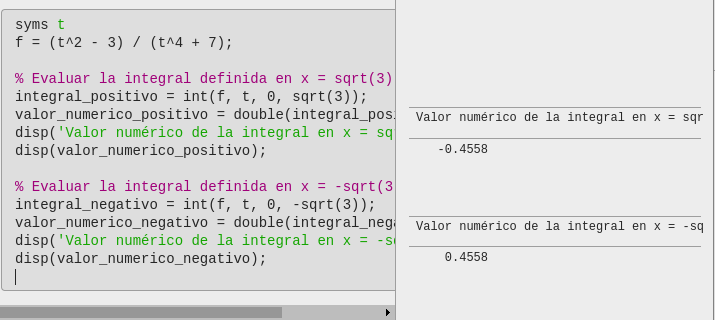
\includegraphics[height = 0.25\textheight]{recursos/ejercicio56.png}\par
\end{figure*}
$\therefore$ Concluimos que  $-\sqrt{3}$ es un máximo absoluto y $\sqrt{3}$ es un mínimo absoluto.

\newpage
d)Graficamos y Concluimos que es correcto
\begin{figure*}[!hbt]
	\centering
	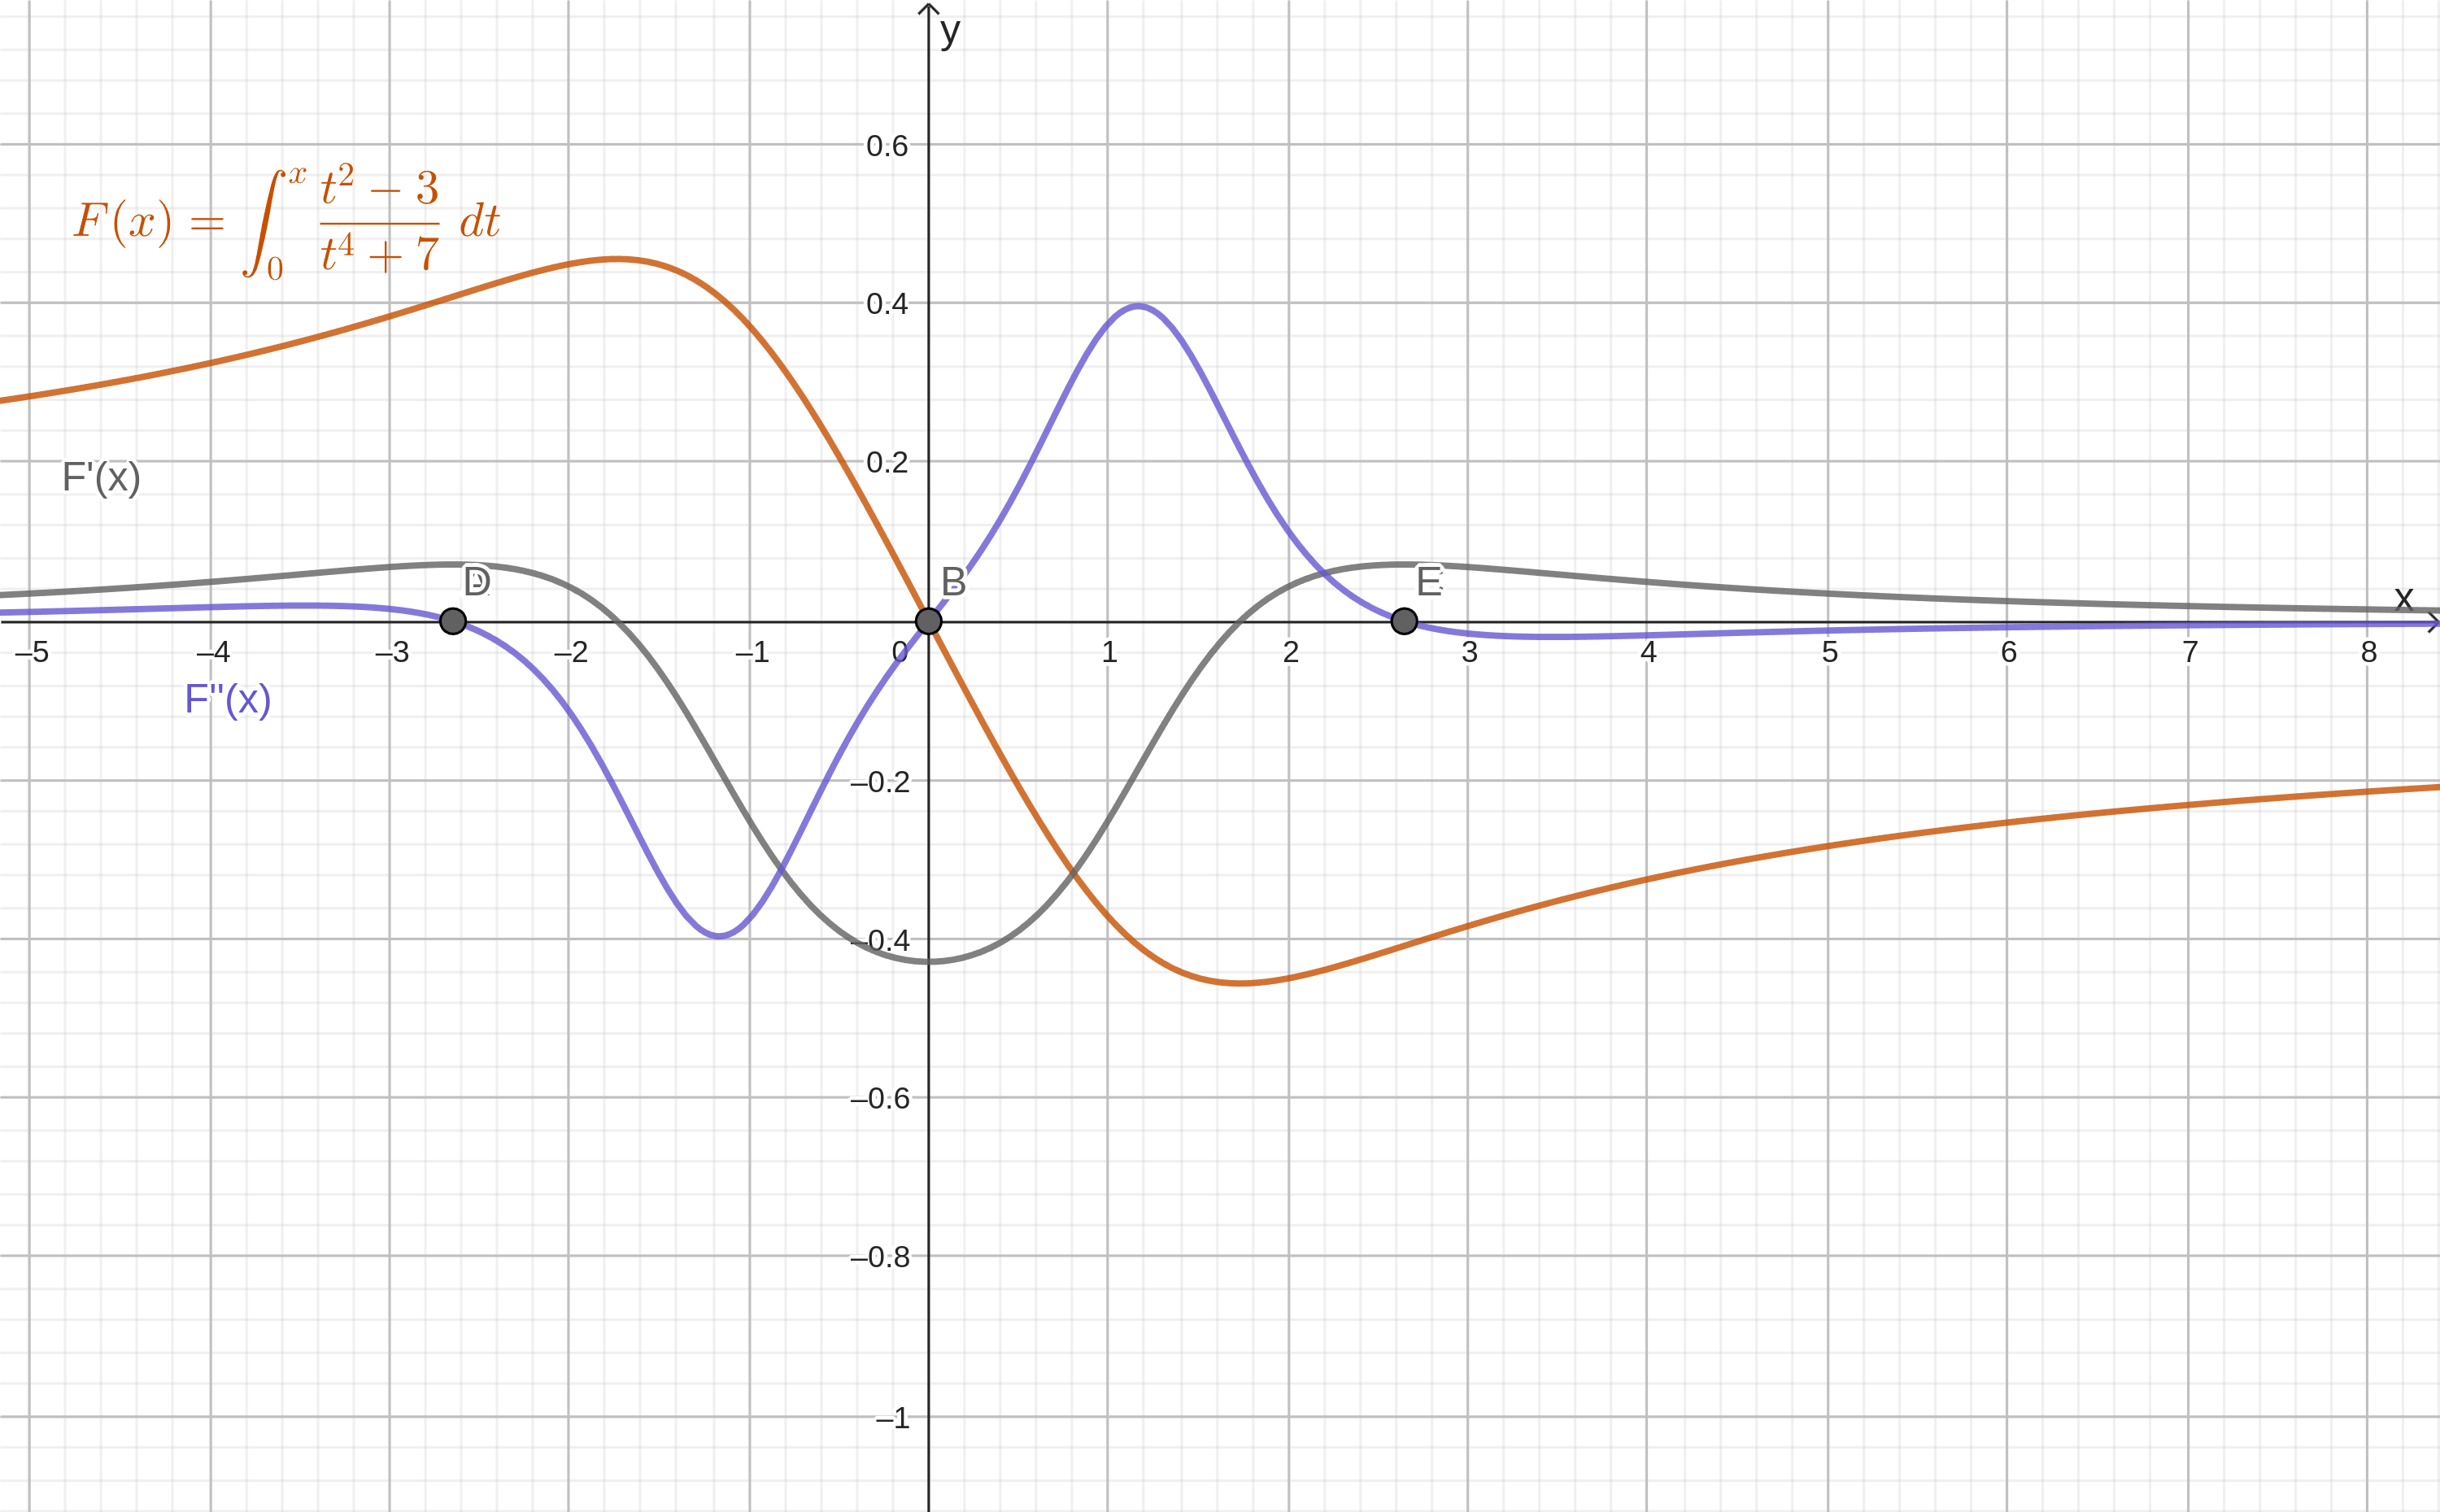
\includegraphics[height = 0.40\textheight]{recursos/ejercicio56_1.png}\par
\end{figure*}